\documentclass[main.tex]{subfiles}
\newcommand\chapterlabel{Ch-entropy}\setcounter{figurenewcounter}{0}\setcounter{tablenewcounter}{0}\setcounter{formulanewcounter}{0}
\setcounter{figurenewcounter}{0}


\begin{document}
\linenumbers
%\setcounter{chapter}{5}
  
\chapter[Entropy and free energy]{Entropy and free energy}
 


      \begin{marginfigure}
      \begin{tikzpicture} \node (a) at (0,0) {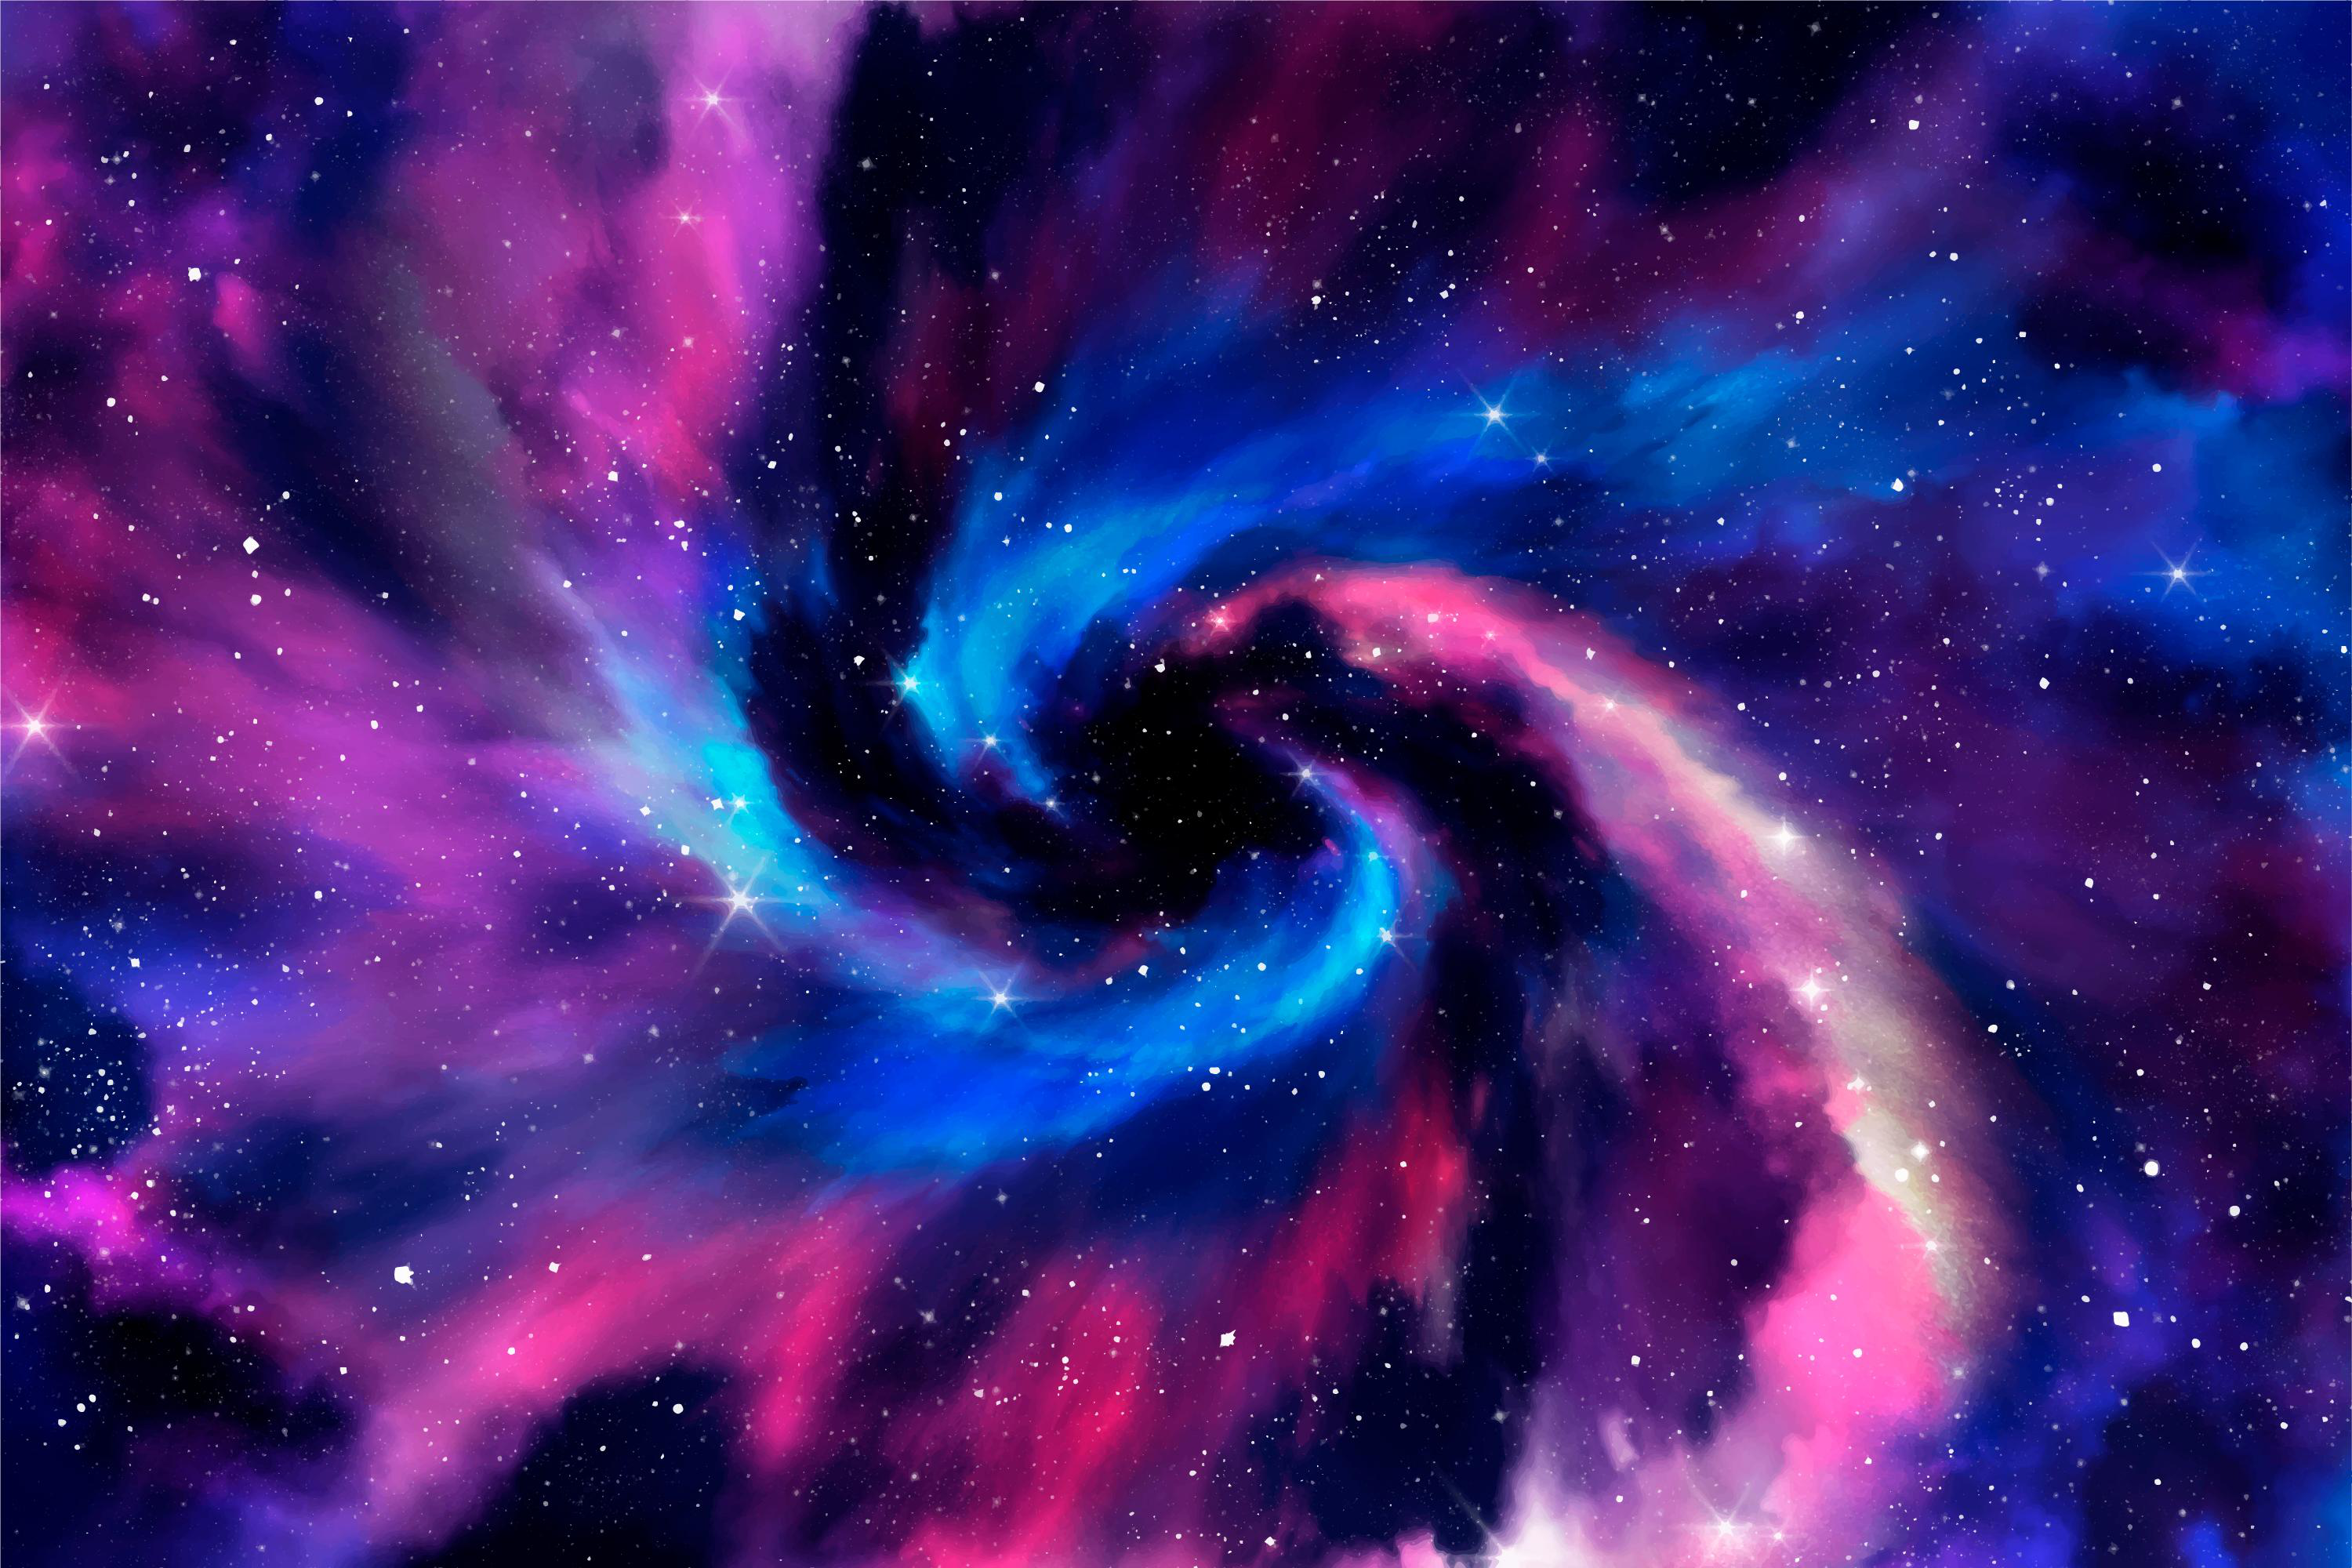
\includegraphics[width=4cm]{../Ch-thermo/figure1}} node[rotate=90, font=\tiny] at ([yshift=.5cm,xshift=.1cm]a.south east) {\textsuperscript{\textcopyright} PxFuel} ;
\end{tikzpicture}
\end{marginfigure}


  \import{files/}{ChapterIntro}


\begin{marginfigure}%LEARNING GOALS BOX
\begin{mytcbox}{GOALS}
\begin{enumerate}[label=\protect\circled{\color{white}\arabic*}]
%\import{files/}{Goal-Spontaneity}
%\import{files/}{Goal-Entropy}						
%\import{files/}{Goal-Calculating-entropy-changes}
\import{files/}{Goal-Standard-molar-entropies}
\import{files/}{Goal-Calculating-entropy-changes-in-chemical-reactions}	
%\import{files/}{Goal-The-second-and-third-law-of-thermodynamics}
\import{files/}{Goal-Gibbs-free-energy	}				
\import{files/}{Goal-Gibbs-free-energy-and-equilibrium}			
%\import{files/}{Goal-Gibbs-free-energy-and-pressure-conditions}		
\end{enumerate}
\end{mytcbox}
\vspace{1cm}
\begin{tcolorbox}[enhanced,colback=red!5!white,colframe=black!50!red,boxrule=1pt,
  arc=0pt,outer arc=0pt,drop heavy lifted shadow]
\faGears\ 
  \import{files/}{ChapterDiscussion}
  \end{tcolorbox}
\end{marginfigure}%LEARNING GOALS BOX

\section{Spontaneity}
\import{files/}{SectionIntro-Spontaneity}
\sloppy\begin{description}
\item[\docfilehook{Spontaneity}{ }] \import{files/}{Subsection-Spontaneity-Spontaneity}
\end{description}




\section{Entropy}
\import{files/}{SectionIntro-Entropy}
\sloppy\begin{description}
\item[\docfilehook{The meaning of Entropy, $S$}{ }]\import{files/}{Subsection-Entropy-The-meaning-of-Entropy}
\item[\docfilehook{A macroscopic description of entropy}{ }]\import{files/}{Subsection-Entropy-Entropy-a-macroscopic-description}
\import{problems/}{SampleProblem1}
\item[\docfilehook{A microscopic description of entropy}{ }]\import{files/}{Subsection-Entropy-Entropy-a-microscopic-description}
\import{problems/}{SampleProblem2}
 \item[\docfilehook{Equivalence between microscopic and macroscopic entropy}{ }]\import{files/}{Subsection-Entropy-Equivalence-between-microscopic-and-macroscopic-entropy}

\end{description}

\section{Standard molar entropies}
\import{files/}{SectionIntro-Standard-molar-entropies}
\sloppy\begin{description}
\item[\docfilehook{Standard molar entropies, $\text{S}^{\circ}$}{ }]\import{files/}{Subsection-Standard-molar-entropies-Standard-molar-entropies}
\import{problems/}{SampleProblem3}
\item[\docfilehook{Factors affecting $S$}{ }]\import{files/}{Subsection-Standard-molar-entropies-Factors-affecting-s}
    \import{problems/}{SampleProblem4}
    \import{files/}{Table-S-and-states-of-matter}
\end{description}
 
  
 \section{Calculating entropy changes }
\import{files/}{SectionIntro-Calculating-entropy-changes}
\sloppy\begin{description}
 \item[\docfilehook{Entropy change and temperature}{ }]\import{files/}{SectionIntro-Calculating-entropy-changes-Entropy-change-and-temperature}
 \item[\docfilehook{Entropy change and volume}{ }]\import{files/}{SectionIntro-Calculating-entropy-changes-Entropy-change-and-volume}
    \item[\docfilehook{Entropy change and pressure}{ }]\import{files/}{SectionIntro-Calculating-entropy-changes-Entropy-change-and-pressure} 
   \item[\docfilehook{Entropy change, pressure and volume}{ }]\import{files/}{SectionIntro-Calculating-entropy-changes-Entropy-change-pressure-and-volume}
    \import{problems/}{SampleProblem5}
   
 \end{description}
 
 
 
 \section{Calculating entropy changes in chemical reactions}\import{files/}{SectionIntro-Calculating-entropy-changes-in-chemical-reactions}
\sloppy\begin{description}
\item[\docfilehook{Standard entropy of reaction, $\Delta \text{S}_R^{\circ}$}{ }]\import{files/}{Subsection-Calculating-entropy-changes-in-chemical-reactions-Standard-entropy-of-reaction}
\item[\docfilehook{Interpreting $\Delta \text{S}_R^{\circ}$}{ }]\import{files/}{Subsection-Calculating-entropy-changes-in-chemical-reactions-Interpreting-S}
\import{problems/}{SampleProblem6}
\item[\docfilehook{Stimate the sign for $\Delta \text{S}_R^{\circ}$}{ }]\import{files/}{Subsection-Calculating-entropy-changes-in-chemical-reactions-Stimate-the-sign-for-S}


\import{problems/}{SampleProblem7}
\end{description}



\section{The second and third law of thermodynamics}\import{files/}{SectionIntro-The-second-and-third-law-of-thermodynamics}
\sloppy\begin{description}
\item[\docfilehook{System, its surroundings and the universe}{ }] \import{files/}{Subsection-The-second-and-third-law-of-thermodynamics-System-its-surroundings-and-the-universe}
\item[\docfilehook{Calculating $\Delta S_{surr}^{T, P}$ }{ }] \import{files/}{Subsection-The-second-and-third-law-of-thermodynamics-Surrounding-S}
\item[\docfilehook{Calculating $\Delta \text{S}_{univ}$: the second law of thermodynamics }{ }] \import{files/}{Subsection-The-second-and-third-law-of-thermodynamics-Universe-S}
\import{problems/}{SampleProblem8}
 \item[\docfilehook{Entropy and equilibrium }{ }] \import{files/}{Subsection-The-second-and-third-law-of-thermodynamics-Entropy-and-equilibrium}
\item[\docfilehook{The third law of thermodynamics }{ }] \import{files/}{Subsection-The-second-and-third-law-of-thermodynamics-3-law}
\import{problems/}{SampleProblem9}
 \item[\docfilehook{The laws of thermodynamics: a review }{ }] \import{files/}{Subsection-The-second-and-third-law-of-thermodynamics-The-laws-of-thermodynamics-a-review}
\end{description}



\section{Gibbs free-energy}\import{files/}{SectionIntro-Gibbs-free-energy}
\sloppy\begin{description}
\item[\docfilehook{Definition of Gibbs free-energy}{ }] \import{files/}{Subsection-Gibbs-free-energy-Defintion}
\item[\docfilehook{Gibbs free-energy and spontaneity}{ }] \import{files/}{Subsection-Gibbs-free-energy-Gibbs-free-energy-and-spontaneity}
\item[\docfilehook{Estimating spontaneity based on the sign of H and S}{ }]\import{files/}{Subsection-Gibbs-free-energy-Estimating-spontaneity-based-on-the-sign-of-H-and-S}
\import{problems/}{SampleProblem10}
\item[\docfilehook{Standard Gibbs free-energy of formation}{ }] \import{files/}{Subsection-Gibbs-free-energy-Standard-Gibbs-free-energy-of-formation}
\import{files/}{Table-G-references}
\item[\docfilehook{Standard free-energy of a reaction, $\Delta \text{G}_R^{\circ}$}{ }] \import{files/}{Subsection-Gibbs-free-energy-Standard-Gibbs-free-energy-of-reaction}
\import{problems/}{SampleProblem11}
\import{problems/}{SampleProblem12}
\end{description}


\section{Gibbs free-energy and equilibrium}\import{files/}{SectionIntro-Gibbs-free-energy-and-equilibrium}
\sloppy\begin{description}
\item[\docfilehook{Gibbs free-energy in equilibrium}{ }]\import{files/}{Subsection-Gibbs-free-energy-and-equilibrium-Gibbs-free-energy-in-equilibrium}
\item[\docfilehook{Gibbs free-energy and phase transitions}{ }]\import{files/}{Subsection-Gibbs-free-energy-and-equilibrium-Gibbs-free-energy-and-phase-transitions}
\import{problems/}{SampleProblem13}
 \hspace{-5cm}\import{files/}{Table-Entropy-phase-change}	

\item[\docfilehook{Gibbs free-energy and work}{ }] \import{files/}{Subsection-Gibbs-free-energy-and-equilibrium-Gibbs-free-energy-and-work}
\end{description}




\section{Gibbs free-energy and pressure conditions}\import{files/}{SectionIntro-Gibbs-free-energy-and-pressure-conditions}
\sloppy\begin{description}
\item[\docfilehook{Impact of pressure on Gibbs free-energy}{ }] \import{files/}{Subsection-Gibbs-free-energy-and-pressure-conditions-Impact-of-pressure-on-Gibbs-free-energy}
\import{problems/}{SampleProblem14}
\item[\docfilehook{Relationship between $\Delta G^{\circ}_R$ and $K_p$}{ }] \import{files/}{Subsection-Gibbs-free-energy-and-pressure-conditions-Relation-between-G-and-K}
\import{problems/}{SampleProblem15}
\end{description}





\import{files/}{Table-thermod-data}




\end{document}
